Блок-схема установки изображена на рисунке \ref{fig:exp_setup}.\par
\begin{figure}[ht]
    \centering
    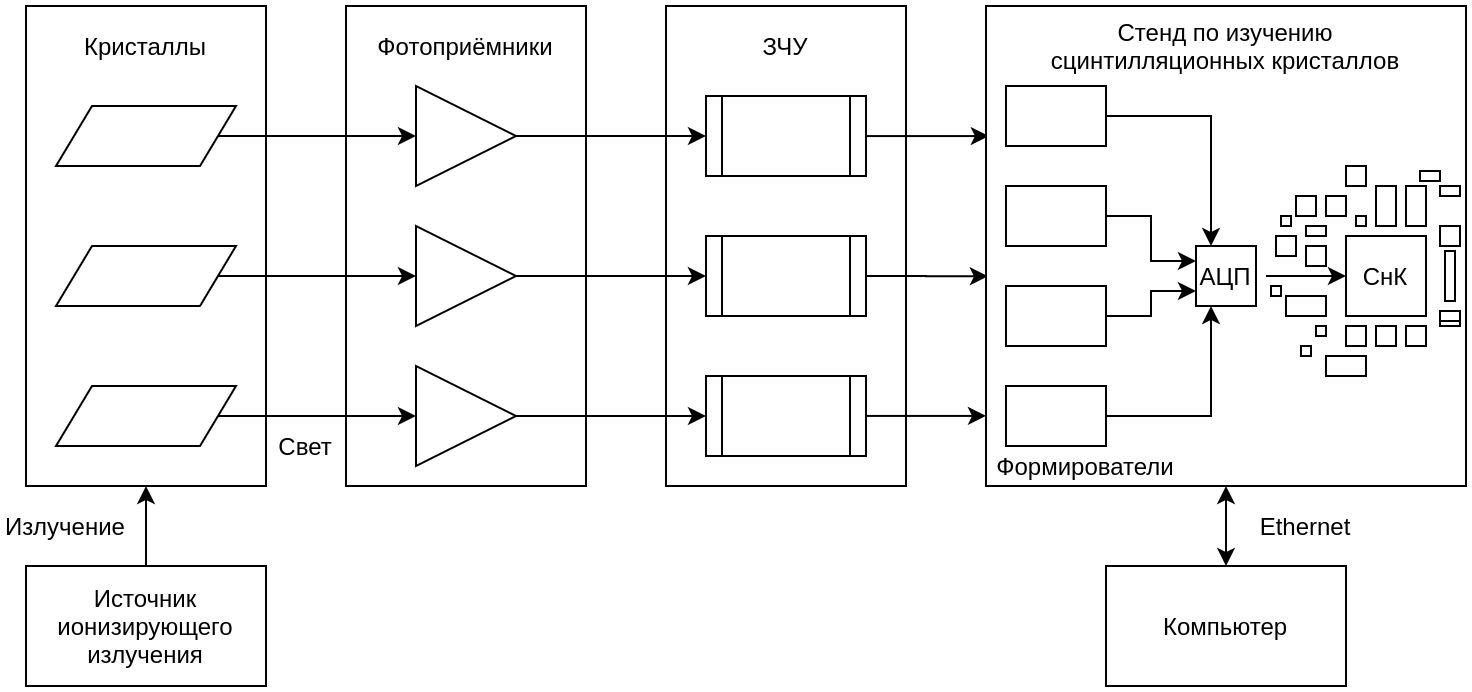
\includegraphics[width=1\linewidth]{Experimental_setup.png}
    \caption{Блок-схема установки}
    \label{fig:exp_setup}
\end{figure}
Ионизирующее излучение с источника попадает на три сцинтилляционных кристалла: исследуемый и два вспомогательных. Излучаемые кристаллами фотоны регистрируются в фотоприёмниках и преобразуются в электрические сигналы. После услиения в зарядо-чувствительных усилителях сигналы подаются на входные каналы стенда, где они обрабатываются. Результат обработки отправляется на компьютер оператора через интерфейс Ethernet. Стенд имеет, кроме основного канала, предназначенного для исследуемого кристалла, два дополнительных для вспомогательных кристаллов.\par
